\documentclass[a4paper, 11pt]{article}

\usepackage[utf8]{inputenc}
\usepackage[T1]{fontenc}
\usepackage[francais]{babel} 
\usepackage{amsmath} % pour les formules de maths
\usepackage{amssymb} % pour des symboles
\usepackage{mathrsfs} % pour avoir acces a des jolies lettres calligrafiées. :)
\usepackage{listings} % pour le code source
\usepackage{color} % pour les couleurs
\usepackage{graphicx} % pour les graphiques (images)
\usepackage{fancyhdr} % pour utiliser le pagestyle fancy
\usepackage[headheight=14pt]{geometry} % pour les marges
\usepackage{hyperref}

\geometry{hmargin=3cm}

\title{TP 0 - Processus stochastiques\\Métaheuristiques pour l'optimisation}
\author{Romain Mencattini}
\date{\today}

\pagestyle{fancy} % pour avoir des entetes et des pieds de page
\renewcommand\headrulewidth{0.6pt}
\fancyhead[L]{Romain Mencattini} % haut de page gauche
\fancyhead[R]{Université de Genève \today} % haut de page droite

\begin{document}
\maketitle
\newpage
\tableofcontents
\newpage

\section{Introduction}
\paragraph{}
Dans ce rapport, nous allons détailler chacun des problèmes, ainsi que les solutions imaginées. Puis nous parlerons des
implémentations au cas par cas. Nous regarderons aussi les résultats obtenus lors des simulations.
Nous avons choisi Python 3.5 pour l'implémentation.

\section{Simulation d'un dé équilibré}
\paragraph{}
On suppose avoir un dé à $N$ faces. On suppose également que ce dé est équilibré, et donc que la probabilité d'une face vaut $\frac{1}{N}$.
La méthode consiste à:
\begin{enumerate}
 \item Générer un nombre aléatoire $r \in [0,1[$
 \item Calculer $i = \lfloor rN \rfloor$
\end{enumerate}

Le $i$ obtenu est donc le résultat du lancé de dé.
La seule difficulté d'implémentation se trouve dans la génération du $r$. Pour ce faire, nous utilisons la méthode $random$ de la librairie
$random$ de Python.
Le comportement de la méthode est définie dans cette documentation : \url{https://docs.python.org/2/library/random.html#random.random}.
Le résultat de $random.random \in [0,1[$.
Le reste du code suit la méthode présentée ci-dessus.
Voici les résultats obtenus:\\
\\
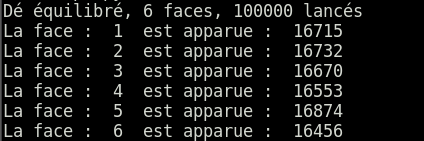
\includegraphics[scale=0.75]{de_equilibre}
On obtient donc des résultats équilibrés.

\section{Simulation d'un dé pipé à l'aide d'un dé équilibré}
\paragraph{}
Dans ce cas, le problème consiste en un dé à $N$ faces mais avec une probabilité d'apparition de $P_i$ pour chaque face.
Voici la méthode proposée dans la série d'exercice:
\begin{enumerate}
 \item On divise le segment en morceau de taille $ppcm(P_i,P_j) \forall i,j in P$ ou P est notre tableau de probabilités.
 \item On fait du pré-processing pour se "souvenir" à quel nombre est associé une case.
 \item On lance le dé équilibré avec $N = length(Tableau)$, ou $Tableau$ est le résultat du pré-processing de l'étape 2
\end{enumerate}

Tout d'abord,nous avons implémenté le ppcm entre deux nombres, puis nous l'avons appliqué à tous les éléments du tableau des $P_i$.
Pour ce faire, nous avons utilisé la fonction $map$ en Python, qui applique une fonction à tous ses éléments.
Sachant que:\\
$ppcm(P_i,P_j) = l$, $ppcm(P_k,l) = res$\\
$ppcm(ppcm(P_i,P_j),P_k) = res$
L'utilisation de $map$ est donc justifiée.\\
Ayant obtenu le ppcm, nous divisons le tableau en morceau de taille $res$.
Puis par une double boucle, nous créons un tableau de sauvegarde, qui va permettre de faire correspondre une case à une chiffre.

Il ne reste plus qu'à lancer le dé avec un $N$ valant la taille du nouveau tableau pour obtenir les résultats.
Voici ce que donne ce programme:\\
\\
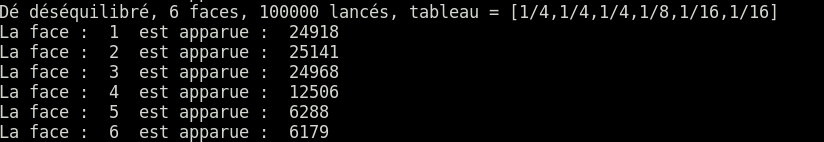
\includegraphics[scale=0.6]{de_pipe_de}
\\
On a plus ou moins la répartition $\frac{1}{4},\frac{1}{4},\frac{1}{4},\frac{1}{8},\frac{1}{16},\frac{1}{16}$\\
Ce qui semble correct.

\section{Simulation d'un dé pipé avec une pièce pipée}
\paragraph{}
Pour fabriquer ce dé pipé à $N$ faces, il nous faut une pièce biaisée.\\
Ces probabilités sont: $p$ pour obtenir un pile, $1-p$ pour face. Soit $r$ notre nombre aléatoire $\in [0,1[$.
On a que si $r < p$ alors c'est l'évènement pile. Face sinon.
Ci-dessous le pseudo-code de l'énoncé:
\begin{enumerate}
 \item On lance une pièce avec une probabilité $p = P_0$ ou $P_0$ est la probabilité de la première case du tableau.
 \item Si c'est pile, on a comme résultat le premier chiffre
 \item Sinon, on normalise la masse de probabilité et on recommence avec le reste du tableau.
\end{enumerate}

Pour normaliser la masse, on fait à chaque étape:
\begin{itemize}
 \item $masse = 1 - P_i$, où $P_i$ est la probabilité utilisée lors du lancer
 \item On divise chaque élément du tableau de probabilité par la masse. On utilise $map$ pour se faire.
 \item On rappelle la fonction jusqu'à ce qu'elle se termine.
\end{itemize}

Nous avons fait le choix d'utiliser une fonction récursive pour la beauté et la compréhensibilité du code. Une version itérative aurait
été bien plus efficace.
Voici les résultats obtenus:
\\
\\
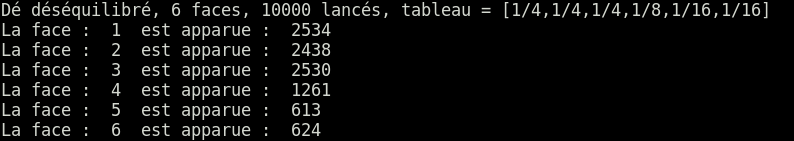
\includegraphics[scale=0.5]{de_pipe_piece}
\\
Les résultats correspondent au tableau de probabilités.

\section{Méthode de la roulette}
\paragraph{}
La méthode de la roulette consiste à:
\begin{enumerate}
 \item calculer le tableau de probabilités cumulées
 \item tire un nombre aléatoire $r \in [0,1[$
 \item choisir la case du tableau tel que: $r > P^{cumul}_i$ pour le plus grand $i$ possible
\end{enumerate}

Nous avons parcouru le tableau de manière linéaire pour trouver le résultat.
Voici ce que donnent cinquante milles lancés:
\\
\\
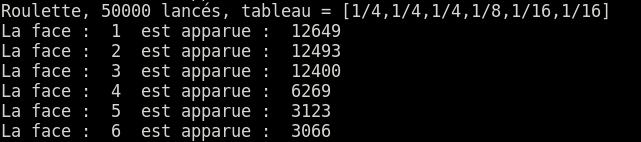
\includegraphics[scale=0.5]{roulette}
\\
On a encore une fois des résultats cohérent avec le tableau de probabilités initial.

\section{Conclusion}
Pour conclure, on peut remarquer que toutes les méthodes donnent des résultats cohérents.
Leurs seules différences se trouvent dans leurs durées d'exécutions ainsi que dans leurs complexités.
\end{document}